% Built by Chapter2/Paper/build_paper_from_chapter2.py -- see PORT_CHANGELOG.md

\section{Introduction}\label{introduction}

Goethite (FeOOH) crystallization is datable only by U-Th/He
geochronology \citep{shustervasconcelos2005,farley2024}. Goethite is a
powerful chronometer for dating surface processes such as weathering and
ferruginization directly: laterite and duricrust formation and
recrystallization \citep{monteiro2014,allard2018,ansart2022}, and the
ferruginization of organic matter and paleosols \citep{heim2006,yappshuster2011,vasconcelos2013,danisik2013,hofmann2017}.

Interpreting a goethite U-Th/He date requires knowing the conditions
under which the mineral retains radiogenic helium. As with any
radiochronometer, meaningful geological interpretation of a measured age
depends on knowing when the system is open to loss or gain of parent or
daughter nuclides. For goethite, step heats of proton-irradiated,
crystalline samples are used to reveal the degree of partial helium loss
by the \textsuperscript{4}He/\textsuperscript{3}He method \citep{shustervasconcelos2005}, and suggest that
helium loss fractions in nature are always non-zero but modest, ranging
from 2 to 30\% \citep{shustervasconcelos2005,heim2006,hofmann2017,deng2017}.
Although one study attempts to explain the variable loss principally as a
result of variable radiation damage \citep{bassal2022}, the effects of
temperature, crystallite size, and chemical composition have not been
determined experimentally and remain unresolved, because goethite
decomposes to hematite (Fe\textsubscript{2}O\textsubscript{3}) in the step
heat experiments used to characterize it \citep{farley2024}.

Laboratory experiments of helium migration under controlled conditions
have proven extremely useful in understanding the mechanisms and rates
of helium migration in geological materials and have produced sensible
results that are predominantly explainable by thermally activated volume
diffusion \citep{reinersfarley1999,farley2000,farley2007,cherniakwatson2011,farley2018}, albeit variably complicated by
the effects of radiation damage and annealing \citep{shuster2006,guenthner2013}. This approach has also been leveraged for
goethite; however, some complications arise when applying this approach
to goethite. Above surface temperatures, goethite decomposes to hematite
and water, often along crystallite elongation directions \citep{goss1987}.
\citet{farley2024} measured evolved water by capacitance manometry during
vacuum step heats and found helium and water release to be tightly
correlated even below 200\textdegree C, indicating that decomposition,
rather than helium migration through an unchanging crystal, governs the
release. Vacuum step-heat results for goethite therefore need not describe
helium behavior in nature.

Still, existing helium step heat measurements of goethite in vacuum
likely remain informative to an extent, as goethite dehydration kinetics
are highly influenced by some of the same factors that could be
responsible for variable helium retention in natural goethite, like
variable grain size \citep{navrotsky2008,guobarnard2011,goss1987}, crystallinity \citep{schwertmann1985} or substitution of
aluminum or other cations within the goethite structure \citep{majzlan2003,bassal2022}. For example, \citet{shustervasconcelos2005} initially
conducted vacuum step-heating experiments on two vitreous,
polycrystalline goethite samples, in which uniformly distributed \textsuperscript{3}He was
introduced by proton irradiation for comparison with radiogenic \textsuperscript{4}He that
was partially lost in nature. The results of \citet{shustervasconcelos2005} could
be well-fit with a model of two distinct diffusion domains or migration
mechanisms with significant differences in helium retention under
surface conditions, e.g. crystallite interiors and intergranular space.
Although these results may have been impacted by dehydration in vacuum,
certain aspects may remain applicable to helium loss in goethite in
nature if helium loss in nature and the laboratory advance through the
samples with similar geometries. One important point is that if
laboratory experiments degas domains in order of their helium
retentivity in nature, even if the rates of loss are affected by
goethite dehydration, then a \textsuperscript{4}He/\textsuperscript{3}He
experiment in vacuum can still be used to measure helium loss \citep{shustervasconcelos2005,vasconcelos2013}.

An additional complexity is that natural goethite almost always occurs
as aggregates of minute crystallites with cross-sections smaller than 1
\textmu m in nature. Neglecting to account for multiple diffusion domains can
lead to inaccurate determinations of activation energy
(E\textsubscript{a}) and frequency factor
(D\textsubscript{o}/a\textsuperscript{2}) for helium diffusion \citep{farley2018}. Detailed step-heating with temperature cycling, as has been done
for hematite \citep{farleyflowers2012,farley2018}, is needed to
characterize domain size and activation energy for polycrystalline
samples.

Goethite dehydration is suppressed at high water pressure \citep{langmuir1971,navrotsky2008}, so a step heat conducted under water vapor saturated conditions may interrogate helium loss
rather than decomposition kinetics. Until now, no studies have reported
helium step-heating results for goethite under water vapor saturated conditions, which could help stabilize goethite or
slow its decomposition to illuminate the processes relevant to helium loss
in natural settings. If
experimental conditions can be controlled to slow the decomposition of
goethite such that the rate of natural helium loss in goethite greatly
exceeds the rate of goethite decomposition into hematite and water, it
would open up an experimental approach to systematically assess how
factors like crystallite size, temperature, radiation damage, and
chemical composition could affect helium mobility and retentivity in
nature \citep{bassal2022}.

Early trials of the method were encouraging (\S\ref{sem-study-of-thermally-treated-polycrystalline-goethite}).
SEM imagery taken of thermally treated natural goethites in vacuum and
open air showed the development of contraction cracks on the outside and
throughout the interior of goethite grains heat treated in vacuum and in
open air (Fig.~\ref{fig:ch2-sem}b,d), while goethite heat-treated when
encapsulated with water did not form cracks (Fig.~\ref{fig:ch2-sem}c).
Goethite heat treated in open air turned red, whereas goethite heat
treated in vacuum remained black.

We test this premise with the first helium step heat experiment on goethite under
water-saturated conditions, and compare it with published vacuum step heats of the same sample
(\S\ref{sec:gt_vacuum}--\ref{sec:gt_hydro}). A thermodynamic and kinetic analysis of goethite
dehydroxylation then explains why water has this effect
(\S\ref{sec:gt_nucleation}).

\begin{figure}[htbp]
\centering
\begin{subfigure}[t]{0.48\textwidth}
  \centering
  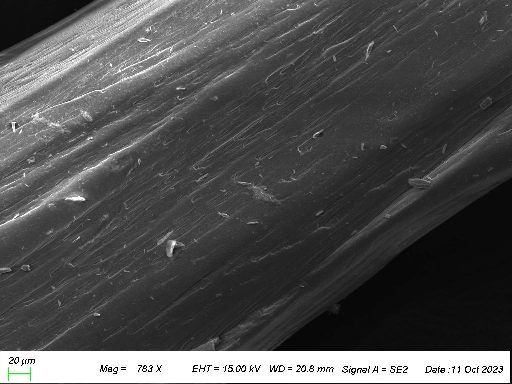
\includegraphics[width=\textwidth]{bahiaGoeControl_20um4.pdf}
  \caption{Control}
\end{subfigure}\hfill
\begin{subfigure}[t]{0.48\textwidth}
  \centering
  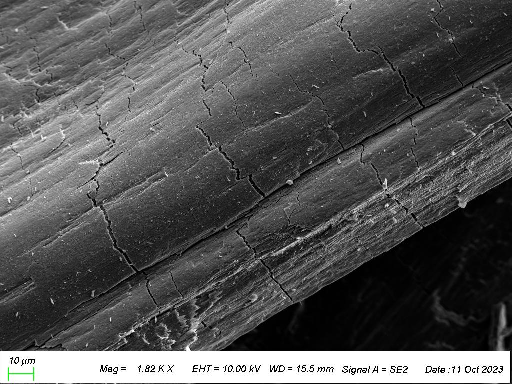
\includegraphics[width=\textwidth]{Goethite_Vac_300C_11hr_10umB0.pdf}
  \caption{Vacuum, 300\textdegree C, 11 h}
\end{subfigure}

\vspace{6pt}
\begin{subfigure}[t]{0.48\textwidth}
  \centering
  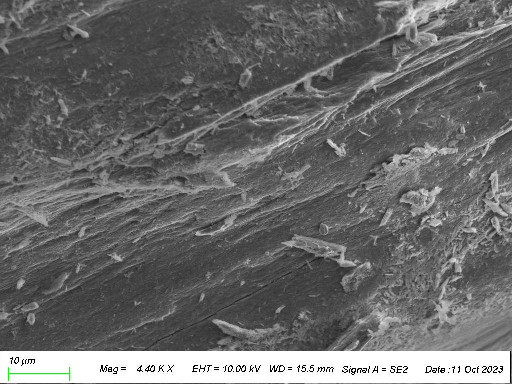
\includegraphics[width=\textwidth]{Goeth_Water_300C_4hr_10um6.pdf}
  \caption{Water-buffered, 300\textdegree C, 4 h}
\end{subfigure}\hfill
\begin{subfigure}[t]{0.48\textwidth}
  \centering
  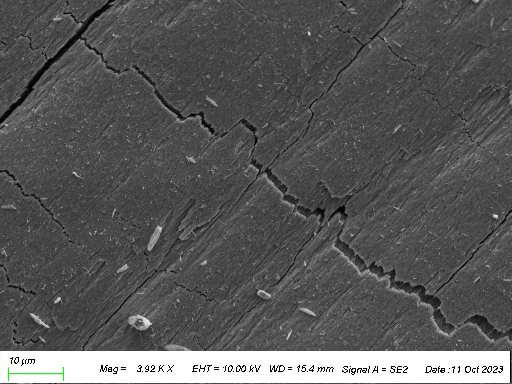
\includegraphics[width=\textwidth]{Goethite_Vacuum_300C_11hr_10u9.pdf}
  \caption{Vacuum, 300\textdegree C, 11 h}
\end{subfigure}
\caption{Secondary electron images of Bahia goethite aggregate before and after heat treatment at 300\textdegree C. (a) Untreated control grain; it has some rough surfaces and rare long-axis-parallel cracks. (b) After 11 hours in vacuum, cracks developed both parallel and perpendicular to the long axis of the polycrystalline aggregate, representing volume contraction due to dehydration/decomposition of goethite into hematite. (c) After 4 hours in a sealed glass tube with water, no cracks indicative of dehydration were visible; most of the aggregate's surface was smoother than the area pictured, which had the roughest texture on the grain. A very small crack parallel to the long axis may indicate some dehydration had occurred, or it may have been inherited from before treatment at water vapor saturation, as observed in the control. (d) The vacuum-heated grain of (b) at the same scale as (c), showing rough cracks at various scales both parallel and orthogonal to the long axis; these are the typical decomposition features that would be expected in (c) if significant decomposition had occurred there.}
\label{fig:ch2-sem}
\end{figure}

\section{Methods}\label{ch2-experimental-methods}

This study builds upon previous helium step heat studies of the dense
colloform goethite sample Win-06-01b (occasionally referred to as
Win0601b) collected within float at the Flinders Ranges in South
Australia \citep{waltenberg2012,monteiro2017}. It yields one of the
oldest known goethite U-Th/He ages: 180-135 Ma \citep{waltenberg2012}.
To
produce a homogeneous distribution of \textsuperscript{3}He, Win-06-01b was irradiated
with 220 MeV protons for 24 hours at the Francis H. Burr Proton Therapy
Center, Massachusetts General Hospital, following standard procedures
\citep{shuster2004} and subsequently was subjected to helium step
heat measurements in vacuum by \citet{monteiro2017} and \citet{farley2024}.
Although these two studies used subtly different heating schedules,
the results of \citet{farley2024} clearly agree well with \citet{monteiro2017}.

In this study, an aliquot of the same irradiated Win-06-01b goethite
used by \citet{monteiro2017} and \citet{farley2024} was encapsulated with
MilliQ water within a silica glass tube following \citet{thyer2026method}. The ampoule retained all of its water through the experiment, including more than a week at
250°C with an internal vapor pressure of about 40~bar \citep{haar1984} (SI Fig.~\ref{fig:ch2-ampoule-post}).

The sealed ampoule, now referred to as HT-Win-06-01b, was placed in a
copper foil packet and mounted to a K-type thermocouple within an
ultra-high vacuum projector lamp heating cell described in more detail
by \citet{farley1999}. Before the experiment began, the ampoule was
loaded in the lamp cell, pumped to high vacuum, and was held at 70°C for
4 days to degas atmospheric helium entrained within the ampoule.

HT-Win-06-01b was subjected to multiple prograde-retrograde heating
cycles to investigate possible MDD behavior. Step durations varied from
2 hours to about a week; the total experiment was conducted over about
40 days and included experimental steps ranging from 170-250°C. We
elected not to heat the sample hotter out of an abundance of caution, because
similar ampoules explode above 300$^{\circ}$C \citep{thyer2026method}.

Recorded temperatures oscillated by \textasciitilde1°C around each target. We 
believe that the recorded temperatures are accurate: encapsulated Durango apatite 
heated in the same way reproduces published diffusivities \citep{thyer2026method}.

Helium isotope measurements of evolved gases from water vapor saturated step heats of glass-encapsulated irradiated HT-Win-06-01b goethite were
acquired at Caltech on a Thermo Fisher
Helix-MC-Plus\textsuperscript{10K} mass spectrometer in peak hopping
mode from January 31\textsuperscript{st}, 2024 to March
13\textsuperscript{th}, 2024. Helium was purified by exposing evolved
gases to a charcoal trap held in liquid nitrogen, a titanium sponge
getter, then a SAES NP10 getter before freely expanding into the
Helix-MC-Plus\textsuperscript{10K}. \textsuperscript{3}He was measured with a
pulse-counting electron multiplier, while \textsuperscript{4}He was detected on a Faraday
detector. Measurements of high \textsuperscript{3}He MM gas standard were analyzed every 8 hours
(totaling 116 measurements) to track instrumental drift of \textsuperscript{3}He and \textsuperscript{4}He
sensitivities and to quantify internal reproducibility.

A cold blank was measured at the beginning of the experiment, showing a
negligible \textsuperscript{3}He blank and a \textsuperscript{4}He blank signal
corresponding to about 1.25 pccSTP, which was similar to \textsuperscript{4}He values
attained during low temperature permeation step measurements. Permeation
steps were thus assumed to measure shifting \textsuperscript{4}He blanks during the
experiment.

For the final step, the HT-Win-06-01b ampoule was broken and dried
overnight in a 50°C oven, then completely degassed by heating to
\textasciitilde1100 °C in a resistance furnace. The final step
measurement was conducted on a Thermo Fisher Helix SFT mass spectrometer. Blank, re-extract and sensitivity details are given in the SI (\S\ref{sec:ch2-si-finalstep}).

Helium released by the sample reaches the mass spectrometer only after permeating the ampoule
wall, so each measured step yield lags the true release. Step yields were corrected for this
permeation lag with the bounding method of \citet{thyer2026method},
which gives lower-bound, central and upper-bound values for every step. The correction and the
ampoule permeabilities measured during the experiment are described in the Supplementary
Information (\S\ref{sec:ch2-si-permeation}). The propagation of the permeation-lag bounds into apparent
diffusivities and isotope ratios are described by \citet{thyer2026thesis}.

\subsection{Kinetic and Diffusive Reductions of Step-Heat Data}\label{sec:gt_kin_methods}

We reanalyzed the published vacuum step heats of irradiated Win-06-01b by \citet{farley2024} (hereafter \emph{KAF}) and
\citet{monteiro2017} (hereafter \emph{HDM}), together with the water-saturated step heat of this study, by reducing every step
both as an apparent first-order conversion rate constant and as an apparent diffusivity.
For the kinetic reduction,
\textsuperscript{3}He is assumed to be immediately released from the goethite lattice upon conversion to hematite, except for a fraction $\phi=0.101$ 
that is inherited by the hematite product. $\phi$ is empirically determined from the \textsuperscript{4}He/\textsuperscript{3}He spectra, corresponding to
the onset of the slow, late "Stage 3" helium loss as described by \citet{farley2024}. The kinetic inversions (Eq.~\eqref{eq:gt_stepk}) 
for the latest steps are highly sensitive to the choice of $\phi$ and are excluded from the fits of the kinetic parameters. 
The KAF steps run with the liquid nitrogen trap isolated are also excluded from the Arrhenius regression.
The fraction of helium released in each step is then $F_i = (1-\phi)\,\alpha_i$, where $\alpha_i$ 
is the fraction of goethite converted in step $i$.

We describe the kinetics of goethite dehydroxylation with a first-order rate law,
\begin{equation}
  \frac{d\alpha}{dt} = k(T)\,(1-\alpha),
  \qquad
  k(T) = A\exp\!\left(-\frac{E_a}{RT}\right),
  \label{eq:gt_F1}
\end{equation}

For a schedule of isothermal steps of duration $\Delta t_j$ at $T_j$, Eq.~\eqref{eq:gt_F1}
integrates to
\begin{equation}
  \alpha_i = 1 - \exp\!\left[-A\sum_{j\le i},\Delta t_j \exp\!\left(-\frac{E_a}{RT_j}\right)\right],
  \label{eq:gt_F1_cum}
\end{equation}

Inverting Eq.~\eqref{eq:gt_F1_cum} step by step gives an apparent rate constant for every
step that is independent of any fitted parameter except $\phi$:
\begin{equation}
  k_i = -\frac{1}{\Delta t_i}\ln\frac{1-\alpha_i}{1-\alpha_{i-1}},
  \qquad \alpha_i = \frac{F_i}{1-\phi}.
  \label{eq:gt_stepk}
\end{equation}

For comparison, the diffusion parameter of each step is obtained with the same
\citet{fechtigkalbitzer1966} inversion for a sphere (Fig.~\ref{fig:gt_arrhenius}). 
A thermodynamic and kinetic model of goethite dehydroxylation, used in
\S\ref{sec:gt_nucleation} to interpret the effect of water in this experiment, is described in the SI
(\S\ref{sec:eqm-thermo}--\ref{sec:gt_nuc_si}).

\subsection{Multiple Diffusion Domain and Thermal History Modeling}\label{sec:gt_mdd_methods}

Together, the $^3$He release and the bulk-normalized $^4$He/$^3$He spectrum constrain the thermal history, if the activation energy
for diffusion is known \citep{farleyflowers2012}. We interpret the data from HT-Win-06-01b in two stages. First, the diffusion
domain structure of the sample is inverted from the $^3$He release alone. Second, natural thermal histories are fitted to the
$^4$He/$^3$He spectrum with that domain structure held fixed. Fits for $N=1$--5 domains and the best-fitting thermal histories
are given in the SI (\S\ref{sec:ch2-si-mdd}).

\paragraph{Diffusion domain structure} Following \citet{farleyflowers2012}, the sample is represented by $N$ non-interacting
spherical domains that share the activation energy of the Stage~1 regression (\S\ref{sec:gt_ht_results}). Each domain holds a
fraction of the uniformly distributed, proton-induced $^3$He at a size relative to the reference domain of the Stage~1
regression ($r/r_0$), giving $2N-1$ free parameters. These minimize the summed squared misfit of the fractional and cumulative $^3$He
yields, weighted equally, over the 28 steps with more than 0.1~pccSTP of $^3$He. The gas released in the six low-signal steps
still counts toward the cumulative yields of later steps, and their durations toward the heating schedule. Domains are added
one at a time, each search starting from the $(N-1)$ domain solution, for $N \in [1,10]$. The Arrhenius and delta plots are not 
fitted, but follow from applying the \citet{fechtigkalbitzer1966} inversion to the model cumulative release. 
Their misfit is reported as a reduced $\chi^2$ over the same 28 steps.

\paragraph{Thermal histories} Given a fixed domain structure, any given thermal history predicts a $^4$He/$^3$He spectrum and a 
bulk He age following \citet{shusterfarley2004}, assuming U and Th are uniformly distributed.
We compare two types of thermal histories: steady cooling with two free parameters and burial then exhumation with 
three free parameters. 
\begin{itemize}
  \item \textbf{Steady cooling:} goethite crystallizes at an elevated temperature $T_0$ at
  formation age $t_\mathrm{form}$ (e.g. in a hydrothermal environment) and linearly cools to 25\,\textdegree C today. 
  \item \textbf{Burial and exhumation:} goethite crystallizes at the surface (20$^{\circ}$C) at formation age $t_\mathrm{form}$. 
  It is buried and linearly heated, reaching a peak temperature T_\mathrm{max} at time $t_\mathrm{peak}$. 
  It is then exhumed to the surface by the paleogene: it is linearly cooled to (20$^{\circ}$C) at 50~Ma. This model roughly 
  follows the thermal history \citet{gibsonstuwe2000} and \citet{mitchell1998} interpreted for the region from apatite 
  fission track thermochronometry. 
\end{itemize}
Each path is scored by the $\chi^2$ misfit of its predicted $^4$He/$^3$He spectrum to the observed spectrum over 
the \MDDNfit{} steps that have more than 0.1~pccSTP of $^3$He,
taking each uncertainty as half the range between the lower- and upper-bound ratios. The reduced
$\chi^2$ uses $\nu=22$ degrees of freedom for steady cooling and $\nu=21$ for burial and exhumation.
$\chi^2$ is evaluated for these free parameters along regularly spaced grids to produce a likelihood 
heatmap (Fig.~\ref{fig:ch2-mdd-heatmaps}). The measured He age range (130--180~Ma; \citealt{waltenberg2012}) 
is treated as a hard constraint. The best fit of each family is
the lowest-$\chi^2$ path with a predicted age in that range.

\subsection{SEM Study of Thermally Treated Goethite}\label{sem-study-of-thermally-treated-polycrystalline-goethite}

In early trials of the ``glass tube method'' for helium step heat
experiments with controlled microenvironments presented here,
sub-samples of goethite morphologically similar to Win-06-01b from
Igarapé Bahia \citep{shustervasconcelos2005,monteiro2017} were heated in
vacuum using the projector lamp heating apparatus of \citet{farley1999}
and in sealed glass ampoules with water additionally added to
provide moisture to slow/prevent dehydration of goethite. All samples
were held at 300°C for 4-11 hours, and the glass ampoules were broken
and the goethites were allowed to air dry before all samples were placed
on carbon tape and carbon coated. These samples were imaged at Caltech
in secondary electron mode by the ZEISS 1550VP Field Emission SEM.

\section{\texorpdfstring{Results }{Results }}\label{ch2-results}

\subsection{Water-Saturated Step Heat of HT-Win-06-01b}\label{sec:gt_ht_results}

The diffusivities determined from the step heat $^3$He and $^4$He
yields for HT-Win-06-01b are always significantly lower than the
diffusivities determined from step heat experiments on the same sample
in vacuum, and they evolve distinctly from those in vacuum. The Arrhenius plot of the $^3$He diffusivities
initially follows a declining concave-up trend until \textasciitilde3.5\%
cumulative $^3$He yield, then slowly decreases in sub-parallel arrays
during prograde and retrograde heating cycles from 3.5-7\% cumulative
$^3$He yields (Fig.~\ref{fig:ch2-arrhenius-zoom}, Fig.~\ref{fig:ch2-delta-zoom}). The Arrhenius plot of the $^4$He diffusivities
differs in shape: it is concave-down to about 5\% cumulative $^3$He yield,
after which it follows a roughly linear array about one log unit below
the $^3$He array (Fig.~\ref{fig:ch2-arrhenius-zoom}). The $^3$He diffusivities settled into a
linear array which was suitable for linear regression after
\textasciitilde7\% of the cumulative $^3$He yield was lost (Fig.~\ref{fig:gt_arrhenius}b). All
remaining diffusivity measurements of the experiment were included in
the linear regression, so that diffusivities from $^3$He loss fractions of
about 7-15\% were included. The linear regression yields an
R\textsuperscript{2} of \ChTwoRtwo, an activation energy of \ChTwoEa ± \ChTwoEaErr
kJ/mol, and a closure temperature of \ChTwoTc ± \ChTwoTcErr °C assuming a cooling
rate of 10°C/Ma and considering only the uncertainty in the regression
intercept (D\textsubscript{0}/a\textsuperscript{2}).

\begin{figure}[htbp]
\centering
\includegraphics[width=0.8\textwidth]{winsor_goethite_Diffusivities_Arrhenius_Zoomin.pdf}
\caption{Linear regression of the last \ChTwoN\ measurements of $^3$He diffusivities in HT-Win-06-01b defining the 
``Stage 1'' reference line. Apparent diffusivities at water vapor saturation are approximately seven natural log units 
lower than in vacuum. A diffusion domain corresponding to the Stage 1 reference line has a closure temperature of 
\ChTwoTc$\pm$\ChTwoTcErr\textdegree C assuming a cooling rate of 10\textdegree C/Ma. Apparent diffusivities calculated from 
$^4$He step heats converge to a linear array a single natural log unit lower than $^3$He. Six steps with $^3$He yields below 0.1 pccSTP 
are omitted for clarity.}
\label{fig:ch2-arrhenius-zoom}
\end{figure}

A delta plot was generated using the intercept and slope parameters from
the $^3$He regression as a reference line, similarly to previous work
\citep{farley2018}. The $^3$He apparent diffusivity delta values monotonically
decrease until a cumulative $^3$He loss of 7\%, after which the delta
values are within error of the reference line (Fig.~\ref{fig:ch2-delta-zoom}). 
\begin{figure}[htbp]
\centering
\includegraphics[width=0.8\textwidth]{DeltasWinsorGTzoomin_VacuumHydrothermal.pdf}
\caption{Delta plot similar to those presented in \citet{farley2018}, or r/r0 plots in \citet{lovera1991} and \citet{farleyflowers2012}. 
Six high uncertainty steps with $^3$He yields below 0.1 pccSTP are omitted for clarity. For visual continuity, the gap left 
behind is bridged with no uncertainty shown. $^3$He monotonically decreases until settling 
on the reference line from 7--15\% $^3$He fractional yield. \textsuperscript{4}He diffusivities and delta values are generally highly uncertain but 
initially show an increase in delta values that settles to a slow increase or plateau about one log unit below the \textsuperscript{3}He reference 
line by a \textsuperscript{3}He fractional yield of 5\%, which is consistent with diffusive loss of radiogenic \textsuperscript{4}He in variably retentive domains. 
Apparent diffusivities for helium in Win-06-01b at water vapor saturation are up to 7 log units lower than the same sample in 
vacuum.}
\label{fig:ch2-delta-zoom}
\end{figure}

\subsection{Kinetic Reanalysis of Vacuum Step Heats}\label{sec:gt_kin_results}

\begin{figure}[htbp]
\centering
\includegraphics[width=\textwidth]{arrhenius_reaction_vs_diffusion.pdf}
\caption{The $^3$He release of every step of the two vacuum step heats of Win-06-01b (red circles:
KAF, \citealt{farley2024}; orange squares: HDM, \citealt{monteiro2017}) and of the water vapor saturated step heat of this study (blue diamonds), reduced in two ways: (a) as first-order conversion rate
constants $k_i$ (Eq.~\eqref{eq:gt_stepk}, $\phi=\ChTwoKinPhi$), and (b) as
apparent diffusivities $D/a^2$ for a sphere \citep{fechtigkalbitzer1966}. Only the filled points are used for the linear regressions. 
Large pink circles mark the two KAF steps with the
LN$_2$ trap isolated. Six low-signal steps of the water-saturated experiment are excluded for clarity. The black line is a first-order Arrhenius fit to filled points of both vacuum experiments. These fitted parameters are given in Eq.~\eqref{eq:gt_line}. 
Below $\sim$180~$^\circ$C both vacuum experiments depart from the first-order line.}
\label{fig:gt_arrhenius}
\end{figure}

All steps are plotted in Fig.~\ref{fig:gt_arrhenius}, for both the kinetic and diffusion reductions, but the fits use only KAF steps \ChTwoKinWinKAF{}
(\ChTwoKinWinKAFT~$^\circ$C) and HDM steps \ChTwoKinWinHDM{} (\ChTwoKinWinHDMT~$^\circ$C).

An unweighted least-squares fit of $\ln k_i$ against $1/T_i$ for the \ChTwoKinLineN{} steps in the fitting window
gives
\begin{equation}
  E_a = \ChTwoKinLineEa \pm \ChTwoKinLineEaErr~\mathrm{kJ\,mol^{-1}},
  \qquad
  \ln A = \ChTwoKinLineLnA \pm \ChTwoKinLineLnAErr
  \label{eq:gt_line}
\end{equation}
Fitting KAF and HDM separately ($\ChTwoKinKAFEa\pm\ChTwoKinKAFEaErr$ and $\ChTwoKinHDMEa\pm\ChTwoKinHDMEaErr$~kJ\,mol$^{-1}$)
or fitting all steps ($\ChTwoKinAllFOneEa$~kJ\,mol$^{-1}$) gives consistent results (\S\ref{sec:gt_supp_mech}).

KAF steps 1--4 and HDM steps 2--7
(below $\sim$180~$^\circ$C) release $^3$He 0.5--3 orders of magnitude faster than the extrapolated 
conversion rate (Fig.~\ref{fig:gt_arrhenius}). This component amounts
to less than 2\% of the $^3$He.

In two KAF steps the trap was isolated and evolved water accumulated in the line. At
230~$^\circ$C the step rate constant fell to \ChTwoKinTrapSuppLow{} times the mean of its neighbors at the same
temperature, and at 240~$^\circ$C to \ChTwoKinTrapSuppHigh{} times. The rate recovered fully when the trap was
restored. We return to these two steps in \S\ref{sec:gt_nucleation}, where they calibrate the nucleation model.

\section{Discussion}\label{ch2-discussion}

\subsection{Dehydroxylation Kinetics in Vacuum Step Heats of Win-06-01b}\label{sec:gt_vacuum}

\citet{farley2024} showed that evolved helium in vacuum step heats of goethite is controlled 
by the process of dehydroxylation to hematite. Here, we present a reanalysis of the vacuum step heat data of Win-06-01b 
from KAF and HDM to show that the helium release of Win-06-01b in vacuum is better described 
by a model of first-order reaction kinetics for goethite dehydroxylation than by a second order diffusion model.

The kinetic reduction yields simpler, more interpretable Arrhenius plots for the vacuum experiments than the diffusion inversion 
does. The kinetic inversion collapses the
prograde steps at the beginning of the vacuum experiments onto a smooth decay to a single line that the diffusion reduction instead shows 
as an irreversible increase in diffusivity (Fig.~\ref{fig:gt_arrhenius}). This initial helium release is most easily read from 
the kinetic inversion as 
a diffusion-related loss from a broad distribution of small, poorly retentive domains in the goethite that is faster
than the rate of dehydroxylation. This is not obvious from the Arrhenius plot produced with the diffusion reduction. 
This shift in the dominance from diffusive loss to dehydroxylation-related loss offers a clear explanation for the 
change in behavior between ``Stage 1'' and ``Stage 2'' in vacuum step heat experiments described by \citet{farley2024}.

Thermogravimetric studies report somewhat higher apparent activation energies for goethite
dehydroxylation ($154\pm15$ to $169\pm8$~kJ\,mol$^{-1}$; \citealt{goss1987}), plausibly because
dehydroxylation kinetics depend on particle size, morphology, and aluminum content
\citep{langmuir1971,yapp1983,tardy1985,majzlannavrotsky2003}.

\subsection{Helium Release under Water-Saturated Conditions Is Diffusive}\label{sec:gt_hydro}

The goal of this work was to attempt to slow the goethite dehydroxylation process
enough to observe thermal helium loss in unchanging goethite.
The thermal schedule included several prograde-retrograde heating cycles
which together would have completely dehydroxylated goethite in vacuum, using the vacuum kinetics of
Eq.~\eqref{eq:gt_line}. Even so, only 14.7\% of the $^3$He was released in the water-saturated experiment.
We argue below that the helium loss in the water-saturated experiment is controlled by diffusion rather than by conversion.

Fig.~\ref{fig:gt_arrhenius} compares the kinetic and diffusion inversions of the step heat data.
These plots show the opposite trend for the vacuum and water vapor saturated experiments. While the vacuum experiments
yield simpler, more interpretable arrays with the first-order inversion, the water vapor saturated experiment collapses into a simpler, coherent
linear array with the diffusivity reduction. The kinetic inversion of the water-saturated data shows a continuously 
declining $k$ for any given temperature as the experiment proceeds, forming a zig-zag pattern. This is the expected behavior 
for a second-order (diffusion-controlled) process for which helium loss 
slows more strongly than a first-order process as the experiment proceeds. 

We consider two alternative mechanisms, recrystallization and fluid-mediated conversion, that might have contributed to the water-saturated release.
Poorly crystalline goethite is known recrystallize under hydrothermal conditions at timescales similar to this experiment 
\citep{schwertmann1985}. Additionally, we induced a fluid-mediated reaction that transformed synthetic goethite pigment to 
hematite at similar temperatures and timescales to this experiment (SI, \S\ref{sec:gt_pigment}). This mechanism of reaction 
is not described by the solid-state nucleation model of \S\ref{sec:gt_nucleation}. We observed that goethite 
either entirely reacted or remained unchanged in this experiment, suggesting that the reaction was fast when it occurs. Either
process would likely release essentially all of the helium in the material it affects. A gradual 
reaction would then make helium release track the extent of reaction, a first-order-like behavior
that the water-saturated data do not show (Fig.~\ref{fig:gt_arrhenius}a), and episodic reaction would
produce abrupt excess release in individual steps, which is also not observed
(Figs.~\ref{fig:ch2-arrhenius-zoom} and~\ref{fig:ch2-delta-zoom}). Their contribution is therefore
likely to be small. If either mechanisms contributed, the apparent diffusivities reported here
would represent upper bounds for diffusion in goethite.

While it is difficult to prove that decomposition or recrystallization is not
playing a role in the results presented in this work, the results presented here point most strongly to
a second-order process (likely volume diffusion) as the dominant mechanism of helium loss for 
Win-06-01b goethite in water-saturated conditions.

\subsubsection{Isothermal Discrimination Test at 250~$^\circ$C}\label{sec:gt_hold_results}

Sequences of isothermal steps can be particularly powerful in discriminating first and second order processes.
Diffusion slows quickly as the diffusion front moves inward, depleting the grain
rims of helium, whereas the rate of first-order conversion slows less for similar fractional yields. We leveraged this 
principle to conduct a sensitive test
by performing a series of 4 consecutive, long isothermal steps at 250~$^\circ$C at the end of the water-saturated experiment: three consecutive 5-hour steps and one 170.8-hour step. Using the first three
5~h steps at 250~$^\circ$C, we invert for both kinetic rate constants and apparent diffusivities, then use each model to project the yield for the 170.8~h step.

Both the first-order and diffusion models yield reproducible results for the three 5-hour calibration steps (Fig.~\ref{fig:gt_hold}), but their 
projections sharply diverge for the long step. Diffusion projects a final fractional cumulative yield of $F = 0.149$ against 
an observed $F = 0.146$, a much stronger agreement than the first-order model prediction of $F = 0.173$, which overpredicts
the helium yield for that step by 46\% (Fig.~\ref{fig:gt_hold}).

\begin{figure}[htbp]
  \centering
  \includegraphics[width=0.65\linewidth]{hydrothermal_hold_projection.pdf}
  \caption{The isothermal 250~$^\circ$C sequence of the water-saturated experiment. Black markers are measured cumulative
  $^3$He fraction. 
  The first-order conversion and spherical volume diffusion models are each calibrated on the three
  5~h steps (grey band) and projected through the 170.8~h step.}
  \label{fig:gt_hold}
\end{figure}

\subsubsection{Consistency with MDD Systematics}\label{consistency-with-mdd-systematics}

All existing helium step heat data on goethites are from naturally occurring
polycrystalline aggregates with unclear and potentially widely variable
grain sizes \citep{monteiro2017,farley2024}, which likely could
follow MDD systematics \citep{farley2018}. In MDD systems, apparent bulk diffusivities of a homogeneously distributed
diffusant at a single temperature will decrease as an experiment
proceeds. This manifests as a monotonic decrease in a delta or r/r0 plot \citep{lovera1991,farley2018}. 
For the activation energy of \ChTwoEa{}~kJ/mol
retrieved by regression in this work, the homogeneously distributed \textsuperscript{3}He
step heat data show this behavior and monotonically decrease within a delta plot (Fig.~\ref{fig:ch2-delta-zoom}).

The strong plateau of the water-saturated goethite experiment at $\Delta = 0$ (Fig.~\ref{fig:ch2-delta-zoom}) and 
the statistically robust regression over a wide range of fractional cumulative \textsuperscript{3}He yields 
(from 7-15\% $\Sigma F_{^{3}\mathrm{He}}$
with an R\textsuperscript{2} of \ChTwoRtwo) suggest that the frequency
factor (intercept) obtained by this regression may be dominated by a single
diffusion domain for $F_c \ge 7\%$ rather than a mix of diffusion domains as is most
often observed in the apparent diffusivities for polycrystalline
hematite \citep{farley2018}.

A multiple diffusion domain inversion of the $^3$He release (\S\ref{sec:gt_mdd_methods})
tests this claim (Table~\ref{tab:ch2-mdd-domains}; Fig.~\ref{fig:ch2-mdd-domains}).
A single domain cannot fit the release (Arrhenius $\chi^2_\nu=27$), and two domains capture
the high early diffusivities but leave a poor Arrhenius fit ($\chi^2_\nu=3.3$). Three
domains reduce the yield misfit by more than half ($\chi^2_\nu=1.08$). With four, the
smallest domain splits in two and the fit improves slightly further ($\chi^2_\nu=1.00$).
Every domain added beyond four coincides in size with the dominant domain and leaves the
fit unchanged (Fig.~\ref{fig:ch2-mdd-domains}). We therefore adopt four domains as a complete description of the $^3$He data:
\begin{itemize}
  \item 0.57\% of the $^3$He at $r/r_0=6.8\times10^{-4}$;
  \item 0.66\% at $r/r_0=2.9\times10^{-3}$;
  \item 1.5\% at $r/r_0=0.031$;
  \item 97.2\% at $r/r_0=1.12$.
\end{itemize}
The three small domains, holding 2.8\% of the $^3$He in total, are fully degassed during the
experiment and account for the high early diffusivities and the gradual approach of the
delta plot to the Stage~1 line (Fig.~\ref{fig:ch2-mdd-arrh-delta}). The dominant domain releases
12\% of its $^3$He during the experiment and diffuses at 0.80 times the Stage~1 rate.
The four-domain model reproduces the Arrhenius array, including its
retrograde segments, and the delta plot (Fig.~\ref{fig:ch2-mdd-arrh-delta}). Fits for
$N=1$--5 are shown in the SI (Fig.~\ref{fig:ch2-si-mdd-3he-fits}).

\begin{figure}[htbp]
\centering
\includegraphics[width=0.7\textwidth]{mdd_free/absolute/chapter/ch2_mdd_domains.pdf}
\caption{Domain structure for the best-fitting multiple diffusion domain models when 1-10 domains are fit to
the $^3$He release of HT-Win-06-01b.
Symbol area scales with the square root of the $^3$He fraction; the dashed line marks the
Stage~1 reference domain. The three small domains are unchanged from $N=4$ onward; domains
added beyond $N=4$ coincide in size with the dominant domain.}
\label{fig:ch2-mdd-domains}
\end{figure}

\begin{figure}[htbp]
\centering
\includegraphics[width=\textwidth]{mdd_free/absolute/chapter/ch2_mdd_arrh_delta_N4.pdf}
\caption{(a) Arrhenius plot and (b) delta plot (departure from the Stage~1 line) of the
measured $^3$He diffusivities of HT-Win-06-01b, with the values implied by the four-domain
fit to the $^3$He yields. Neither plot is fitted directly but is a consequence of the fit to the 
$^3$He cumulative and fractional yields. The six low-signal steps are omitted.}
\label{fig:ch2-mdd-arrh-delta}
\end{figure}

\subsection{Why Water Suppresses Dehydroxylation}\label{sec:gt_nucleation}

Under the vacuum kinetics of Eq.~\eqref{eq:gt_line}, the water-saturated heating schedule would have
converted the sample completely many times over ($\sum_i k_{\mathrm{vac}}(T_i)\,\Delta t_i \approx \ChTwoKinSumKdt$). Even if
all of the observed $^3$He release came from conversion ($\alpha = \ChTwoKinHTAlphaObs$), the conversion rate
at water saturation can be at most $10^{\ChTwoKinLogRObs}$ times the vacuum rate, and at most
$10^{\ChTwoKinLogRDetect}$ times for conversion to stay below 1\%. A thermodynamic and
classical-nucleation model of goethite dehydroxylation accounts for this suppression (SI,
\S\ref{sec:eqm-thermo}--\ref{sec:gt_nuc_si}). Goethite is unstable relative to hematite and water both in
vacuum and at water saturation (SI Fig.~\ref{fig:gt_PT}), but water is a product of the reaction and exerts
strong control over the reaction's driving force $\Delta\mu$. In the vacuum of a step-heating line the water
pressure approaches zero and $\Delta\mu$ is unbounded; at water saturation $\Delta\mu$ is only 6--11~kJ per mole
Fe$_2$O$_3$, 1.6--2.4 times $RT$ (SI Table~\ref{tab:gt_dmu}). Because the barrier to nucleating hematite
within goethite scales as $\gamma^3/\Delta\mu^2$ \citep{turnbull1949}, it vanishes in vacuum, consistent
with the simple Arrhenius behavior observed in both vacuum experiments, but this nucleation barrier is present at saturation. 
We calibrate the model's one free parameter, an effective interfacial energy ($\gamma_{\mathrm{eff}} =
\ChTwoKinMCGammaMid$~J\,m$^{-2}$), using the relative reaction rates at two known partial pressures of water from 
the vacuum experiment of \citet{farley2024} (\S\ref{sec:gt_kin_results}). From this calibration follows the nucleation barrier
of \ChTwoKinBarSat~$k_BT$ at water saturation and 250~$^\circ$C. The predicted fractional conversion over the water-saturated 
schedule given this barrier is $10^{\ChTwoKinMCCNTLo}$ to $10^{\ChTwoKinMCCNTHi}$ (95\% uncertainty interval): essentially 
predicting no appreciable reaction to occur. This explanation applies to solid-state (topotactic) conversion; fluid-mediated reaction 
lies outside it (\S\ref{sec:gt_hydro}).

\subsection{\texorpdfstring{High Helium Retentivity of
Win-06-01b-HT}{ High Helium Retentivity of Win-06-01b-HT}}\label{high-helium-retentivity-of-win-06-01b-ht}

The apparent diffusivities of the water-saturated experiment are approximately seven natural log units lower than
those obtained from the same sample in vacuum by \citet{monteiro2017} and \citet{farley2024} (Fig.~\ref{fig:gt_arrhenius}b,
Fig.~\ref{fig:ch2-arrhenius-zoom}, Fig.~\ref{fig:ch2-delta-zoom}). This high
helium retentivity is explored through two lenses: closure temperature
of cooling samples \citep{dodson1973} and isothermal diffusion \citep{wolf1998}.

If the slope and intercept on the regression of \textsuperscript{3}He apparent
diffusivities from Fig.~\ref{fig:ch2-arrhenius-zoom} are taken to represent a real
diffusion domain, then it has a closure temperature of \ChTwoTc ± \ChTwoTcErr °C assuming a cooling rate of 
10°C/Ma and considering uncertainty only in the intercept D\textsubscript{0}/a\textsuperscript{2} \citep{dodson1973}.
The multiple diffusion domain inversion (\S\ref{consistency-with-mdd-systematics}) indicates
that the dominant domain, which holds 97\% of the $^3$He, diffuses at 0.80 times the rate of
the Stage~1 line. Its closure temperature is correspondingly about 1.6\,\textdegree C higher,
well within the closure temperature's uncertainty, so the Stage~1 parameters are used throughout this section.

Goethite is most often formed near Earth's surface and thus U-Th/He geochronology
is most typically applied to date surface processes \citep{heim2006,yappshuster2011,vasconcelos2013,danisik2013,monteiro2014,hofmann2017,allard2018}. 
For crystals of goethite grown and collected near the surface, 
the concept of a closure temperature is poorly applicable, as
it necessarily assumes a cooling rate \citep{dodson1973}. In such cases, a
better measure of retentivity is an analysis of isothermal retentivity
over time \citep{wolf1998}, which is commonly expressed in terms of
t'/t, where t' is the helium age and t is the isothermal holding time
(often the `real age'). For an isothermal holding time of 100 Ma at
40°C, a diffusive domain with the parameters obtained from the
regression of \textsuperscript{3}He apparent diffusivities of Win-06-01b-HT yields t'/t = 0.968, 
where t' and t are helium age and isothermal holding time, respectively. At 25°C, this domain is nearly
quantitatively retentive of helium even at billion-year time scales (t'/t $\approx$ 1). 

This study of a single sample has no bearing on potential complexities
related to aluminum content, radiation damage, or crystal defects on bulk diffusion
\citep{bassal2022}, nor does it permit estimation of the diffusivity
at infinite temperature (D0) which would require experiments on controlled grain sizes.

\subsection{Profiling Radiogenic Helium Loss with $^4He$/$^3He$ Ratios of Win-06-01b-HT}\label{spectra-of-win-06-01b-ht}

Bulk-normalized \textsuperscript{4}He/\textsuperscript{3}He ratios in step heats of irradiated samples
measure the rounding of concentration profiles of radiogenic helium by natural helium loss, if the
loss mechanism in nature and in the laboratory share the same geometry
\citep{shusterfarley2004,farley2024}. Aside from the first
experimental step, bulk-normalized \textsuperscript{4}He/\textsuperscript{3}He ratios for all experiments begin
at vanishingly small values and steeply increase at first, with the rate
of increase slowing as the experiments proceed (Fig.~\ref{fig:ch2-ratio-spectra}). This
behavior is consistent with complete then partial loss of radiogenic
helium in nature in the least retentive domains and is observed in all
step heat experiments on irradiated goethite \citep{shustervasconcelos2005,vasconcelos2013,farley2024}. 
These least retentive domains could represent fine goethite grains, or they could represent 
interstitial helium trapped between crystallite grain boundaries.

The water vapor saturated experiment records lower bulk-normalized \textsuperscript{4}He/\textsuperscript{3}He
ratios than the vacuum experiments at any given $\Sigma F_{^{3}\mathrm{He}}$ for the duration
of the experiment. This suggests that the geometry of helium loss
differs between the water vapor saturated and vacuum experiments. 
If this is the case, then the \textsuperscript{4}He/\textsuperscript{3}He spectra of goethite measured in vacuum may not
straightforwardly encode the thermal history of the sample in the same way that it does
in phases such as hematite or apatite \citep{farleymckeon2015,shusterfarley2004}. 
More \textsuperscript{4}He/\textsuperscript{3}He spectra of goethite at water vapor saturation are needed to 
investigate this hypothesis further. 

\begin{figure}[htbp]
\centering
\includegraphics[width=\textwidth]{Ch2_spectra_combined.pdf}
\caption{Bulk-normalized \textsuperscript{4}He/\textsuperscript{3}He ratios for Win-06-01b goethite step heats 
against cumulative fractional \textsuperscript{3}He yield. The water vapor saturated experiment of this study is black,
with uncertainties shown in grey. The vacuum experiments of \citet{monteiro2017} and \citet{farley2024} are orange and red
respectively. The best age-consistent thermal-history predictions (shown as stars in Fig.~\ref{fig:ch2-mdd-heatmaps}) are
shown here in blue for the burial history with crystallization at 195~Ma, and in freen for the steady cooling history 
(\S\ref{sec:gt_thermal_history}). 
The water vapor saturated experiment shows lower bulk-normalized \textsuperscript{4}He/\textsuperscript{3}He ratios at a 
given $\Sigma F_{^{3}\mathrm{He}}$ for the duration of the experiment, suggesting that 
\textsuperscript{4}He/\textsuperscript{3}He spectra are dependent on the partial pressure of water and that the geometry 
of goethite dehydroxylation differs from the geometry of helium diffusion through goethite. Steps of the water vapor 
saturated experiment  with less than 0.1~pccSTP of \textsuperscript{3}He are omitted. The horizontal axis 
changes scale at $\Sigma F_{^{3}\mathrm{He}} = 0.2$ (double slash) to emphasize the portion of the plot where water 
vapor saturated data exist.}
\label{fig:ch2-ratio-spectra}
\end{figure}


These ratios also bear on the natural thermal history of Win-06-01b. Throughout the range of
$\Sigma F_{^{3}\mathrm{He}}$ that defines the Stage~1 reference line (7--15\%), step \textsuperscript{4}He/\textsuperscript{3}He
ratios remain at 0.67--0.82 of the bulk value (Fig.~\ref{fig:ch2-ratio-spectra}).
Radiogenic \textsuperscript{4}He is depleted relative to the uniformly distributed \textsuperscript{3}He in this domain, 
so even this retentive domain lost helium in nature. A domain with the
Stage~1 parameters is nearly quantitatively retentive at Earth-surface temperatures
(\S\ref{high-helium-retentivity-of-win-06-01b-ht}), so this loss is difficult to attribute to thermally activated
diffusion at surface conditions. Either Win-06-01b experienced temperatures well above surface conditions 
(perhaps it grew in a hydrothermal setting or experienced burial heating), or non-thermal processes such as fluid-mediated
recrystallization caused partial helium loss in nature. Section~\ref{sec:gt_thermal_history}
tests whether thermally activated diffusion alone, within the domain structure inferred from
the $^3$He release, can reproduce the measured spectrum. 

\subsection{Thermal History of Win-06-01b}\label{sec:gt_thermal_history}

To test whether thermally activated diffusion alone can reproduce the measured $^4$He/$^3$He spectrum, 
we explore a subspace of geologically reasonable, yet simple thermal paths. With the four-domain structure of
\S\ref{consistency-with-mdd-systematics} held fixed, we fit steady-cooling and
burial-and-exhumation thermal histories to the $^4$He/$^3$He spectrum of HT-Win-06-01b
(\S\ref{sec:gt_mdd_methods}). Previous studies constrain our exploration of the burial-and-exhumation paths. 
\citet{gibsonstuwe2000,mitchell1998} interpret regional cooling 
from roughly 50--70\,\textdegree C after the mid-Cretaceous from their apatite
fission-track studies. \citet{mitchell1998} additionally interpret, from limited $\sim$1.5~km thick sediment accumulation 
in Triassic intramontane basins, that parts of the ranges were near the surface in the early
Mesozoic.  Table~\ref{tab:ch2-mdd-thermal} gives the best fit of each
family, Fig.~\ref{fig:ch2-ratio-spectra} compares the best steady-cooling and burial
predictions with the spectrum, and Fig.~\ref{fig:ch2-mdd-heatmaps} shows their $\chi^2$ maps on a
common color scale.

\paragraph{Steady cooling} Linear cooling at a rate of $\sim$0.3\,\textdegree C\,Myr$^{-1}$ 
from 78\,\textdegree C at 150~Ma ($\chi^2_\nu=2.00$) to 25\,\textdegree C 
today fits the spectrum best. Such paths pass through
$\sim$55\,\textdegree C at 90~Ma, within constrains set by the apatite fission-track \citep{gibsonstuwe2000,mitchell1998}. 
The spectrum alone without the age constraint prefers somewhat younger, hotter paths: the unconstrained minimum
($\chi^2_\nu=\MDDLinGlobalChi$; \MDDLinGlobalT\,\textdegree C at \MDDLinGlobalTform~Ma) predicts
a He age of \MDDLinGlobalAge~Ma (Fig.~\ref{fig:ch2-mdd-heatmaps}b). 

\paragraph{Burial and exhumation} Burial paths fit the spectrum less well
($\chi^2_\nu=5.0$--6.5), but they agree with the independent regional constraints of \citet{gibsonstuwe2000} and \citet{mitchell1998}. For
crystallization at 180 and 195~Ma, the best age-consistent paths peak at $\sim$60\,\textdegree C at
70 and 80~Ma (Fig.~\ref{fig:ch2-mdd-heatmaps}a). These peaks fall in or just after the apatite
fission-track window, within the 50--70\,\textdegree C range of \citet{gibsonstuwe2000} and at
the $\leq$60\,\textdegree C limit reported by \citet{mitchell1998}. For crystallization at
210~Ma, only hotter and earlier peaks (70--74\,\textdegree C at 105--130~Ma) give an age within
the measured range, and they fit worse ($\chi^2_\nu=6.5$).

Isothermal histories, which constrain only the product of diffusivity and time, cannot reproduce
the shape of the spectrum and are not considered further (Table~\ref{tab:ch2-mdd-thermal}).

\paragraph{Where the families differ} The steady-cooling and burial predictions differ
mainly in the earliest steps ($\Sigma F_{^{3}\mathrm{He}}\lesssim0.035$;
Fig.~\ref{fig:ch2-ratio-spectra}), which sample the outer rim of the dominant domain. On
the burial path the sample sits at 20\,\textdegree C for the last 50~Myr, long enough for
radiogenic $^4$He to re-accumulate in the rim, so the early ratios are overpredicted. Steady
cooling keeps the rim depleted until geologically recent times, with diffusive loss
declining monotonically toward the present. Elsewhere both leave the same residual pattern:
the underpredict $^4$He/$^3$He ratios between $\Sigma F_{^{3}\mathrm{He}}=$~0.04 and 0.06, and overpredict them in
for the two longest high-temperature steps. These fits do not weight steps differently by their fractional yields
except indirectly in that longer steps have tighter uncertainties and thus incur more penalty for a given misfit. 
The trend of the residuals at the end of the experiment suggest that the best fitting thermal history would 
be different if the experiment continued further and more helium was degassed. 

\begin{figure}[htbp]
\centering
\includegraphics[width=\textwidth]{mdd_free/absolute/chapter/ch2_mdd_heatmaps_N4.pdf}
\caption{Reduced $\chi^2$ of the $^4$He/$^3$He spectrum for (a) burial paths with crystallization
at 195~Ma, as a function of the time and magnitude of peak temperature, and (b) steady cooling
to 25\,\textdegree C, as a function of crystallization age and initial temperature. Both panels
share one color scale, anchored to the overall minimum. Dashed lines show the predicted
bulk He age at 130 and 180~Ma. A diamond is placed at the unconstrained best fit for the linear cooling path, 
and stars locate the best fit with a He age within the 130--180 Ma bounds set by \citet{waltenberg2012}.}
\label{fig:ch2-mdd-heatmaps}
\end{figure}

\paragraph{Consistency with diffusive loss} These two families of thermal paths encode very different geologic origins. We 
note that any number of arbitrarily complex thermal paths can be evaluated against the data with 
this workflow, but a thorough search for viable thermal paths is beyond the scope 
of this study, and is an ill-posed exercise for a single sample, for which many potential histories could
fit the data non-uniquely. The main purpose of this exercise is instead to demonstrate that the $^4$He/$^3$He data we 
present here are consistent with diffusive loss of radiogenic helium in nature. We do not claim to 
have found the unique thermal history of the sample, but have demonstrated that plausible thermal histories 
reproduce our results reasonably well. This result suggests that proton-irradiated goethite may be a viable 
target for $^4$He/$^3$He thermochronometry as described by \citet{shusterfarley2004} and applied
to polycrystalline samples by \citet{farleyflowers2012}, especially when multiple samples are 
available to constrain a region's thermal history.

\section{Conclusions}\label{conclusions}

We applied the silica-glass ampoule method of \citet{thyer2026method} to conduct the first
helium step heat experiment on goethite under water-saturated conditions, using
proton-irradiated goethite Win-06-01b, which was previously been step heated in vacuum. The main
findings are:
\begin{enumerate}
  \item Polycrystalline goethite heated with water does not develop the contraction cracks that
  form in vacuum, and the water-saturated helium release differs fundamentally from release in
  vacuum. Published vacuum step heats of Win-06-01b follow first-order conversion to hematite,
  whereas the water-saturated release shows the history and time dependence of diffusion. These
  results are consistent with the interpretation that goethite dehydroxylation was sufficiently kinetically-inhibited 
  to observe helium diffusion through unchanging goethite.
  \item Apparent diffusivities at water saturation are approximately seven natural log units
  lower than those of the same sample in vacuum. Beyond 7\% cumulative $^3$He release they define
  a linear Arrhenius array with an activation energy of \ChTwoEa{}~$\pm$~\ChTwoEaErr{}~kJ/mol, and
  the delta plot follows multiple diffusion domain systematics. A four-domain model places 97\% of
  the $^3$He in a single domain.
  \item Extrapolated to 25\,\textdegree C, this majority domain is essentially quantitatively retentive of
  helium over billion-year timescales, supporting the use of goethite (U--Th)/He dates to date
  surface processes.
  \item The $^4$He/$^3$He spectrum shows that even this retentive domain lost radiogenic helium in
  nature, and thermally activated diffusion can account for that
  loss. Steady cooling from 76--80\,\textdegree C at 150--175~Ma fits the spectrum best, favoring
  crystallization from warm, possibly hydrothermal, fluids. Burial of surface-formed goethite to a
  Late Cretaceous peak of 58--65\,\textdegree C, consistent with regional apatite fission-track
  constraints, remains a viable alternative.
  \item The water-saturated $^4$He/$^3$He spectrum is distinct from the vacuum spectra of
  the same sample, suggesting that dehydroxylation and diffusion may degas goethite with different
  geometries. Vacuum $^4$He/$^3$He spectra of goethite may therefore not encode thermal histories as
  directly as they do for minerals that do not decompose during vacuum step heat experiments.
  \item A thermodynamic and kinetic analysis explains why water preserves goethite on experimental
  timescales. The driving force for dehydroxylation is unbounded at the near-zero water pressure of a vacuum line, but is only
  6--11~kJ at saturation, which raises the barrier to topotactic hematite nucleation enough to suppress conversion over
  experimental timescales.
\end{enumerate}

Fluid-mediated conversion and recrystallization, which transformed synthetic goethite pigment under
similar conditions, would likely degas the affected material completely. These data are most consistent with 
a second-order control, limiting the contribution of fluid-mediated conversion and recrystallization to be small. 
If either contributed, the diffusivities reported here are upper bounds and the retentivity a lower bound. 
Separating the effects of crystallite size, chemical composition, and radiation damage on helium retention 
will require further water-saturated step heats of irradiated goethite of controlled grain size, 
which this approach makes straightforward.

\section*{Data Availability}

The step heat data, permeation-lag bounds, and model outputs supporting this study are archived
on Zenodo \citep{thyer2026data}: \url{https://doi.org/10.5281/zenodo.22113166}.

\section*{CRediT authorship contribution statement}

\textbf{Ben J. Thyer:} Methodology, Investigation, Formal analysis,
Visualization, Writing -- original draft. \textbf{Jonathan Treffkorn:} Methodology,
Investigation. \textbf{Kenneth A. Farley:} Conceptualization, Resources, Supervision, Funding
acquisition, Writing -- review \& editing.

\section*{Declaration of competing interest}

The authors declare that they have no known competing financial interests or personal
relationships that could have appeared to influence the work reported in this paper.

\section*{Acknowledgements}

This work was supported by National Science Foundation (NSF) grant EAR 1945974 to K.A. Farley.
Dr. Hevelyn Monteiro is thanked for her mentorship and resources in support of the SEM work presented here. 

\section*{Declaration of Generative AI and AI-assisted technologies in the writing process}

During the preparation of this work the authors used Claude (Anthropic) to assist with software
programming, and with editing and LaTeX typesetting of the manuscript. After using this tool, the
authors reviewed and edited all content and take full responsibility for the content of
the publication.
